\documentclass[../main.tex]{subfiles}

\begin{document}
	\subsection{Output capacitance influence}
	{
		\begin{tcolorbox}[colback=gray!5!white,colframe=gray!75!black]
			We consider a centered CMOS inverter for which the output $S$ is connected to a charge capacitance $C$. This capacitance $C$ modeled the sum of the capacitance of the input gates addressed by the signal $S$, plus the interconnection capacitance. We now use
			\begin{itemize}
				\item $L_n = 0,6 \mu m$ and $W_n = 3,0 \mu m$;
				\item $L_p = 0,6 \mu m$ and $W_p = 6,0 \mu m$;
			\end{itemize}
			Measure the propagation time $T_p(\text{up} \to \text{down})$ and $T_p(\text{down} \to \text{up})$ for $C$ equal to $0.0pF$, $0.1pF$, $0.2pF$, $0.5pF$ and $1.0pF$.
			
			Plot $T_p(C)$.
		\end{tcolorbox}
		
		We modify the code for the centered inverter to introduce the capacitance $C$. I could not find support for \textit{parameter sweep} in Spice Opus, so we must run the script with a different value of $C$ to measure each propagation time.
		
		\begin{lstlisting}
			.include cmosws.mod
			
			Vin 1 0 pulse(0.0V 3.3V 5ns 1ns 1ns 3ns 8ns)
			Vdd 2 0 dc 3.3V
			M1  3 1 0 0 MODN L=0.6U W=3.0U
			M2  2 1 3 2 MODP L=0.6U W=6.0U
			C1  3 0 0.0pF
			*C1  3 0 0.1pF
			*C1  3 0 0.2pF
			*C1  3 0 0.5pF
			*C1  3 0 1.0pF
			
			.tran 0.05ns 13ns
			.end
		\end{lstlisting}
		
		\begin{figure}[H]
			\centering
			% Subfigure 1
			\begin{subfigure}{0.3\textwidth}
				\centering
				\includegraphics[width=\textwidth]{plots/Q6_0pf.png}
				\caption{$C = 0pF$}
				\label{fig:subfig1}
			\end{subfigure}
			% Subfigure 2
			\begin{subfigure}{0.3\textwidth}
				\centering
				\includegraphics[width=\textwidth]{plots/Q6_01pf.png}
				\caption{$C = 0,1pF$}
				\label{fig:subfig2}
			\end{subfigure}
			% Subfigure 3
			\begin{subfigure}{0.3\textwidth}
				\centering
				\includegraphics[width=\textwidth]{plots/Q6_02pf.png}
				\caption{$C = 0,2pF$}
				\label{fig:subfig3}
			\end{subfigure}
			
			% Subfigure 4
			\begin{subfigure}{0.3\textwidth}
				\centering
				\includegraphics[width=\textwidth]{plots/Q6_05pf.png}
				\caption{$C = 0,5pF$}
				\label{fig:subfig4}
			\end{subfigure}
			% Subfigure 5
			\begin{subfigure}{0.3\textwidth}
				\centering
				\includegraphics[width=\textwidth]{plots/Q6_1pf.png}
				\caption{$C = 1pF$}
				\label{fig:subfig5}
			\end{subfigure}
			
			\caption{Output \textcolor{red}{$V_{out}$ in red} and input \textcolor{green}{$V_{in}$ in green} for different values of $C$}
			\label{fig:mainfig}
		\end{figure}
		
		\begin{table}[htbp]
			\centering
			\renewcommand{\arraystretch}{1.5} % Adjust row height
			\begin{tabular}{|c|c|c|}
				\hline
				$C$ & $T_p(\text{up} \to \text{down})$ & $T_p(\text{down} \to \text{up})$ \\ \hline
				$0pF$ & $0,11ns$ & $0,12ns$ \\ \hline
				$0,1pF$ & $0,52ns$ & $0,62ns$ \\ \hline
				$0,2pF$ & $0,81ns$ & $1,02ns$ \\ \hline
				$0,5pF$ & $1,69ns$ & $1,82ns$ \\ \hline
				$1pF$   & $3,11ns$ & $1,08ns$ \\ \hline
			\end{tabular}
			\caption{Propagation times measured in each plot}
			\label{tab:transition}
		\end{table}
		
		When we plot the propagation times, we observe a clear linear relation between $T_p$ and $C$. We can use linear regression to plot $T_p(\text{up} \to \text{down})$ and $T_p(\text{down} \to \text{up})$. For high values of $C$ however, it is importance to notice that because the capacitor never manages to fully decharge, $T_p(\text{down} \to \text{up})$ starts to decrease and we lose this linear behavior. The plot was made using \textit{Python}.
		
		\begin{figure}[H]
			\centering
			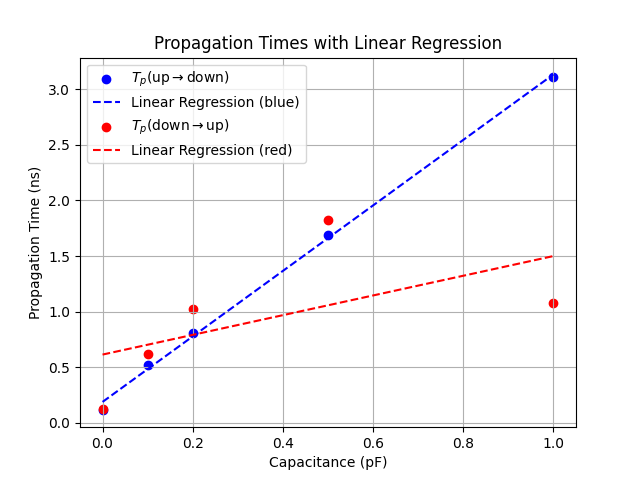
\includegraphics[width=0.5\textwidth]{plots/Q6_plot.png}
			\caption{Propagation time $T_p$ as function of capacitance $C$}
		\end{figure}
		
	}
	
\end{document}